\recipe{American Pancakes}
\label{recipe:american_pancakes}
\worktime{30 minutes}
\totaltime{30 minutes}
\makes{Makes enough for one hungry person}
\source{From Ram (Ask Jack)}

\begin{ingredients}
    \item \SI{200}{\gram} Self raising flour
    \item Baking powder, \SI{1.5}{\teaspoon}
    \item Salt, \SI{0.25}{\teaspoon}
    \item 3 large Eggs
    \item \SI{200}{\milli \litre} Milk
    \item \SI{25}{\gram} butter + extra for cooking
    \ingroup{Topping suggestions}
    \item Maple syrup
    \item Yogurt
    \item Blueberries
    \item Bacon
    \item Whipped cream
\end{ingredients}

\begin{method}
Mix together dry ingredients and wet ingredients separately.

Combine wet ingredients slowly into the dry ingredients.

Fry.
\end{method}


\begin{figure}[h]
  	\centering
  	
  	\begin{tikzpicture}
  		% Save the image in a box to get its dimensions
  		\sbox0{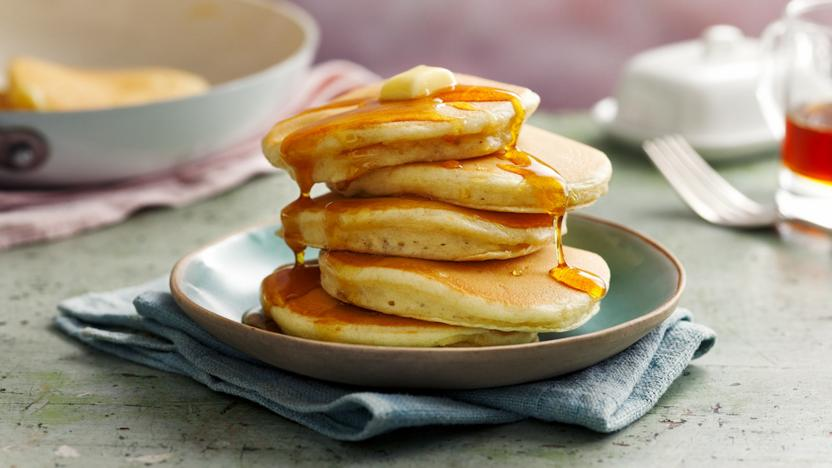
\includegraphics[height=0.5\linewidth]{images/fluffyamericanpancak_74828_16x9.jpg}}%
  
  		% Draw a clipping rectangle with rounded corners
  		\path[clip, rounded corners=0.5cm] (0,0) rectangle (\wd0,\ht0);
  
  		% Place the image inside the clipped area
  		\node[inner sep=0pt, outer sep=0pt, anchor=south west] at (0,0) {\usebox0};
	\end{tikzpicture}

  \caption*{}
\end{figure}